
\section{Introduction à CUBE ProjectAssistant} % Major section
% Example citation \cite{Figueredo:2009dg}. (Literaturangabe; Literaturliste)

Dans ce manuel d'utilisateur, l'abréviation CUBE PA sera utilisée.

\subsection{A quoi sert CUBE PA?} % Sub-section

CUBE PA est un outil de travail pour la gestion de projets. En tant qu'application de banque de données avec accès basé sur le web, CUBE PA peut être utilisé n'importe où et n'importe quand tant qu'une connexion Internet est établie. Il soutient les flux de travail typiques pour la gestions de projets, comme la gestion de séances et d'acquisitions. En plus, il met à disposition toutes les informations relatives à la gestion de projet partout et à tout moment.

\subsection{Qui devrait utiliser CUBE PA ?} % Sub-section

CUBE PA est surtout utile pour des projets qui présentent plusieurs des caractéristiques suivantes :

% \begin{itemize} % - Zu grosser Abstand verwendet
% 	\item xy
% \end{itemize}
	
\begin{compactitem}
	\item Plusieurs parties, organisations et/ou entreprises sont impliquées
	\item Acteurs travaillent depuis différents endroits
	\item Structure complexe avec beaucoup de sous-projets
	\item Longues durées
	\item Beaucoup de séances, d'acquisitions, etc.
	\item Décalage horaire entre les acteurs
	\item Besoin de possibilités de travail flexibles hors bureau, jour et nuit, dans le train, etc.
\end{compactitem}	
		
\ \\
Lorsqu'on décide d'utiliser CUBE PA pour un projet, il est important que si possible toutes les personnes impliquées dans la gestion du projet utilisent CUBE PA. Ceci concerne aussi bien les décideurs que leurs assistants. De cette manière seulement peut-on profiter au maximum de l'effort initial nécessaire pour mettre en place CUBE PA.
	
\subsection{La structure de CUBE PA} % Sub-section

CUBE PA est divisé en plusieurs domaines, décrits ci-dessous, qui correspondent chacun à un élément du menu principal. Les domaines n'ont pas tous le même degré de développement : quelques uns sont bien développés, d'autres sont encore à un stade de développement rudimentaire. D'autres domaines sont également prévus. Chaque domaine est brièvement décrit ci-dessous, afin de donner au lecteur une idée de son but et de son stade de développement. Chaque domaine est ensuite décrit dans un chapitre séparé, qui apporte des informations plus précises sur son utilisation.

\pagebreak
\subsubsection{Le menu de CUBE PA} % Sub-sub-section

\setlength{\abovecaptionskip}{0pt}

\begin{wrapfigure}[15]{l}{7cm}   % [x] Wie manche Zeile soll sich um die Grafik "brechen"
  \vspace{-25pt}      % Grundwert war 20; mit 30 schön oben beim Text ausgerichtet
  \begin{center}
    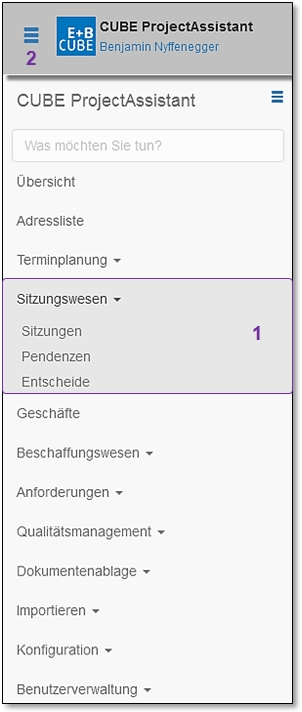
\includegraphics[height=150mm]{../chapters/01_Einfuehrung/pictures/1-3-1_Menuuebersicht_oSitzungswesen.jpg}
  \end{center}
  \vspace{-20pt}
  \caption{Le menu}
  \vspace{-10pt}
\end{wrapfigure}
Les différents domaines de CUBE PA sont accessibles par le menu. Selon le domaine, des sous-domaines différents peuvent être choisis. Cliquez d'abord sur le domaine souhaité. S'il contient des sous-domaines, ceux-ci seront affichés. Dans l'exemple illustré, le domaine „Gestion de séances“ \col{(1)} comporte les trois sous-domaines „Séances“, „Affaires en suspens“ et „Décisions“. Cliquez sur le sous-domaine désiré pour l'ouvrir. Cliquez à nouveau sur le nom du domaine (dans cet exemple : „Gestion de séances“) pour masquer les sous-domaines. 

\vspace{\baselineskip}

En cliquant sur le symbole du menu \col{(2)}, le menu peut être affiché ou masqué. Ceci vous permet d'avoir une surface de travail plus grande. \\

\vspace{7cm}

\textbf{Le menu personnalisé}

\begin{wrapfigure}[7]{r}{5.5cm}
\vspace{-35pt}
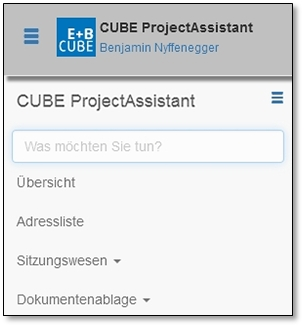
\includegraphics[height=50mm]{../chapters/01_Einfuehrung/pictures/1-3-1_MenuAngepasst.jpg}
\caption{Le menu personnalisé}
\end{wrapfigure}

Selon les autorisations données à un utilisateur (selon les différents rôles, par exemple administrateur), le menu peut varier dans sa diversité / ses éléments visibles par rapport aux prises d'écran dans ce manuel et par rapport à d'autres utilisateurs. Dans le présent manuel, tous les éléments de menu sont représentes.

\subsubsection{L'aperçu}
\label{bkm:Ref132000001}
L'aperçu personnel apparaît directement après la connexion à CUBE PA. Il présente une vue d'ensemble des affaires qui vous concernent directement.

\begin{figure}[H] % Example image
\center{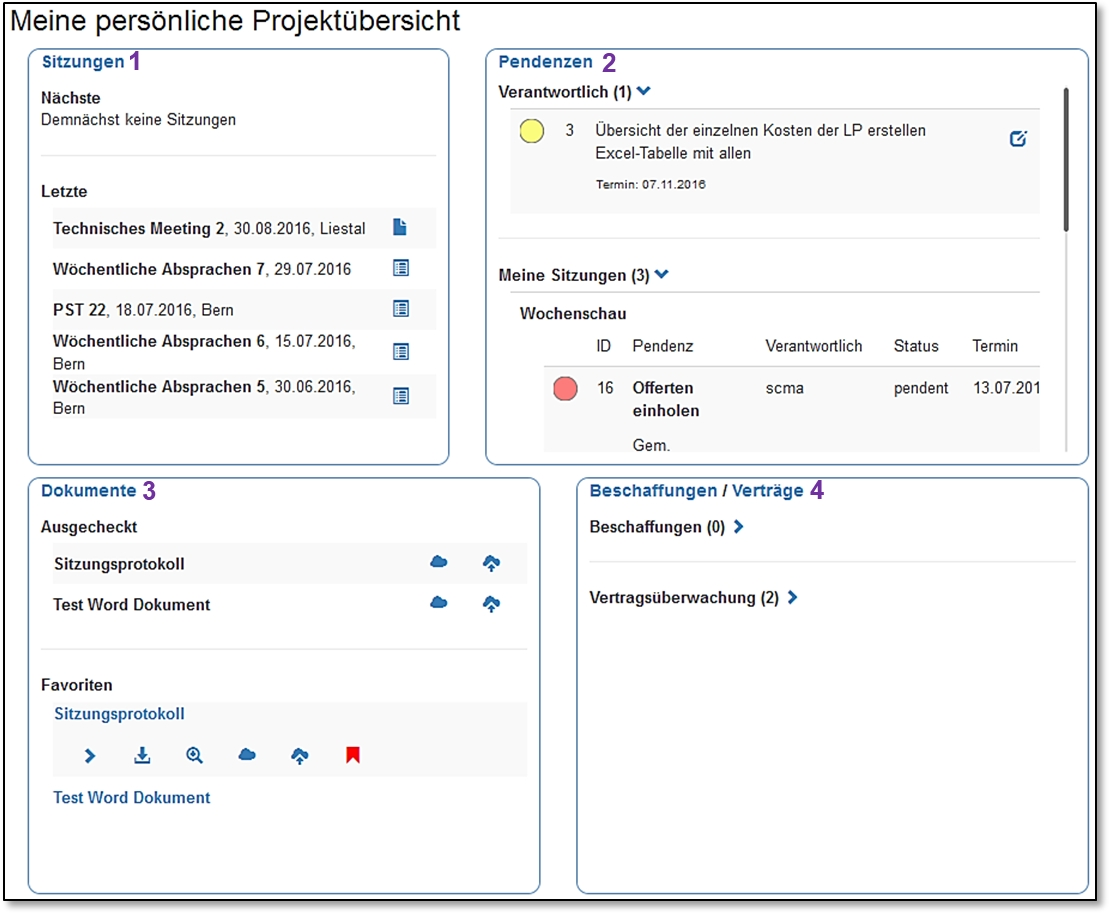
\includegraphics[width=1\linewidth]{../chapters/01_Einfuehrung/pictures/1-3-2_persUebersicht.jpg}}
\caption{Mon Aperçu de Projet}
% \label{fig:speciation}
\end{figure}

Les séances actuelles sont affichées en haut à gauche \col{(1)}. Sous „Suivante“ se trouvent les séances auxquelles vous participez qui prennent place prochainement . Vous pouvez modifier l'invitation pour une séance ou la sauvegarder comme fichier PDF pour ensuite l'envoyer. Sous „Passée“ se trouvent les séances qui ont pris place récemment. Cliquez pour ouvrir le procès-verbal d'une séance passée. S'il n'y a pas encore une version définitive du procès-verbal, vous pouvez modifier la version actuelle. En cliquant sur le titre bleu „Séances“ \col{(1)} vous êtes directement dirigé vers le sous-domaine „Séances“ du domaine „Gestion de séances“.

\vspace{\baselineskip}

En haut à droite sont affichées les affaires en suspens \col{(2)} pour lesquelles vous êtes responsable et celles dans lesquelles vous êtes impliqué (collaboration). Vous pouvez modifier une affaire en suspens en cliquant dessus. Le masque de saisie correspondant s'ouvre. Si vous cliquez sur le titre bleu „Affaires en suspens“ \col{(4)}, vous êtes directement dirigé vers le sous-domaine „Affaires en suspens“ du domaine „Gestion de séances“. Pour plus d'informations sur la création et la modification d'affaires en suspens, consultez les chapitre 5.4 et 5.5, respectivement.

\vspace{\baselineskip}

En bas à gauche sont affichés les documents pertinents pour vous \col{(3)}. Sous „Extraits“ se trouvent les documents que vous avez extraits. Vous pouvez directement ouvrir un document extrait ou le réintroduire. \\

Sous „Favoris“ se trouvent les documents que vous avez marqués comme favoris personnels. En cliquant sur le titre bleu d'un document, les options sont affichées : Vous pouvez télécharger un document favori, voir ses détails, modifier la saisie ou extraire le document pour le modifier pendant qu'il est verrouillé contre les modifications par d'autres utilisateurs. Vous pouvez aussi prévisualiser le document. Si vous n'avez plus besoin d'un document favori, cliquez sur le symbole de drapeau rouge. La saisie disparaît en actualisant la page ou en cliquant sur 'Aperçu'. En cliquant à nouveau sur le titre du document, les options sont  masquées. Si vous cliquez le titre bleu „Documents“ \col{(3)}, vous êtes directement dirigé vers le sous-domaine „Documents“ du domaine „Classement des documents“.

\vspace{\baselineskip}

% Text, welcher bis zur Grafik reichen soll, ist unmittelbar an Grafikeinbettung 
% zu schreiben, dann kommt Grafikeinbettung, dann Text, welcher Grafik umschliesst.

\begin{wrapfigure}{r}{0.5\textwidth}
  \vspace{-20pt}
  \begin{center}
    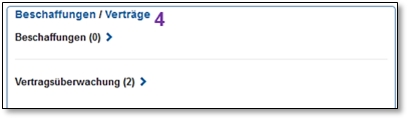
\includegraphics[width=0.5\textwidth]{../chapters/01_Einfuehrung/pictures/1-3-2_persUebersichtBeschaffung.jpg}
  \end{center}
  \vspace{-20pt}
%  \caption{Persönliche Übersicht}
  \vspace{-10pt}
\end{wrapfigure}
En bas à droite sont affichés les acquisitions et les contrôles de contrats \col{(4)} auxquels vous participez et pour lesquels une action de votre part est attendue. Le nombre de saisies qui vous concernent est affiché entre parenthèses. Cliquez sur le symbole de flèche horizontale pour afficher une acquisition ou un contrôle de contrat. Cliquez sur le symbole de loupe près d'une acquisition ou d'un contrat pour directement le modifier. Selon l'état de l'acquisition, il serait plus judicieux d'ouvrir l'option de traitement convenable via le menu, en cliquant sur le domaine „Fonction d'acquisition“ et le sous-domaine correspondant. Pour une description détaillée de la fonction d’acquisition, consultez le chapitre 7. Si vous cliquez le titre bleu „Acquisitions“ ou „Contrats“ \col{(4)}, vous êtes directement dirigé vers le sous-domaine „Acquisitions“ ou „Contrats“ du domaine „Fonction d'acquisition“.

\vspace{\baselineskip}

\begin{wrapfigure}[5]{r}{0.5\textwidth}
  \vspace{-45pt}
  \begin{center}
    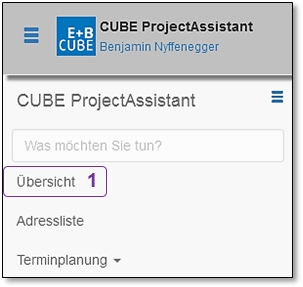
\includegraphics[width=0.4\textwidth]{../chapters/01_Einfuehrung/pictures/1-3-2_MenuepunktUebersicht.jpg}
  \end{center}
  \vspace{-20pt}
  \caption{Aperçu dans le menu}
  \vspace{-10pt}
\end{wrapfigure}
Si vous changez de domaine avec le menu, vous quittez l'aperçu personnel. Pour y retourner, cliquez le l'élément „Aperçu“ \col{(1)} du menu principal.

\pagebreak
\subsubsection{Liste d'adresses} % Sub-sub-section

Dans la liste d'adresses, toutes les personnes (utilisateurs) et entreprises (unités d'organisation) recensées dans CUBE PA sont affichées. Avec la fonction de filtre, les saisies recherchées peuvent être rapidement repérées.

\subsubsection{Planning} % Sub-sub-section

Cette fonctionnalité est pour l'instant encore dans un stade rudimentaire et se limite essentiellement au téléchargement de documents. Pour cette raison, cette fonctionnalité n'est pas décrite dans les détails. Le 'Planning détaillé' en une fonction d'importation de documents Microsoft-Project (fichiers xml), qui permet également de filtrer et d'afficher les données importées.

\subsubsection{Gestion de séances} % Sub-sub-section

CUBE PA soutient tous les flux de travail liés aux séances, notamment l'invitation aux séances et la rédaction de leurs procès-verbaux. Par contre, CUBE PA ne gère pas les rendez-vous dans les calendriers et la réservation de salles de conférence, qui se font normalement avec Outlook. Les données saisies pour l'invitation à une séance sont automatiquement disponibles comme base pour le procès-verbal de la séance. Ce dernier peut être directement saisi dans CUBE PA et corrigé par les participants.

\subsubsection{Transactions} % Sub-sub-section

CUBE PA permet de gérer un journal de projet simple et structuré. Quand ce journal est consciencieusement géré, tous les participants sont tenus au courant du déroulement du projet, partout et à tout moment.

\subsubsection{Fonction d'acquisition} % Sub-sub-section

CUBE PA permet de gérer le flux de travail entier lié à une acquisition, de sa publication à l'adjudication, en passant par le contrôle des offres. Les liens entre la publication de l'offre, les offres, et les contrats sont faciles à suivre grâce à un système de numérotation intelligent. Pour l'instant, seule la fonctionnalité d'acquisition avec un soumissionnaire (procédure de gré à gré) est implémentée. La fonctionnalité pour des acquisitions avec plusieurs soumissionnaires suivra dans la prochaine phase de développement.

\subsubsection{Exigences} % Sub-sub-section

Cette fonctionnalité est pour l'instant encore dans un stade rudimentaire et est essentiellement limitée au téléchargement de documents. Elle n'est donc pas décrite en détail.

\subsubsection{Gestion de la qualité / Manuels} % Sub-sub-section

Cette fonctionnalité est pour l'instant encore dans un stade rudimentaire et est essentiellement limitée au téléchargement de documents. La fonctionnalité 'Manuels' permet la saisie de manuels de projet ou d'autres manuels dans CUBE PA.

\subsubsection{Classement des documents} % Sub-sub-section

Le classement des documents permet de classer toute sorte de document en versions. Les documents classés peuvent être identifiés avec des métadonnées / tags (étiquettes). En plus de la possibilité d'extraire et réintroduire des documents et de les modifier directement dans les programmes Office (comme avec Microsoft SharePoint), les documents peuvent aussi être visualisés en ligne (fonction de prévisualisation). Chaque document peut être attribué à un lieu géographique (double-clic directement dans Google Maps). Le lieu peut aussi être changé ultérieurement par glisser-déposer (drag-and-drop) dans la carte. Le classement des documents permet ainsi d'avoir un aperçu des documents qui sont géographiquement proches.

\subsubsection{Fonction d'importation} % Sub-sub-section

Cette option permet d'importer des données d'échéanciers et de transactions dans CUBE PA.

\subsubsection{Configuration} % Sub-sub-section

La configuration sert à recenser des données spécifiques au projet qui vont apparaître plus tard dans des listes de sélection. Comme ce travail est normalement effectué par peu de personnes, la configuration n'est décrite que brièvement.

\subsubsection{Gestion des utilisateurs} % Sub-sub-section

Dans la gestion des utilisateurs, les différents utilisateurs, équipes et groupes sont recensés et gérés.
